\documentclass[11pt]{article}
\usepackage{mathtools}
\usepackage{mdframed}
\usepackage{fullpage}
\usepackage{enumitem}
\usepackage{amsfonts}
\usepackage{tikz}
\usepackage{graphicx}
\usepackage{fancyhdr}
\usepackage{lastpage}


%edit this for each class
\newcommand\name{John Collin Vincent}
\newcommand\classname{Coms 486}
\newcommand\assignment{Assignment 2}


\newcounter{excounter}
\setcounter{excounter}{1}
\newcommand\ques[2]{\vskip 1em  \noindent\textbf{\arabic{excounter}\addtocounter{excounter}{1}.} \emph{#1} \noindent#2}
\newenvironment{question}{\ques{}\begin{quote}}{\end{quote}}
\newenvironment{subquestion}[1]{#1) \begin{quote}}{\end{quote}}

\pagestyle{fancy}
\rfoot{\name, page \thepage/\pageref{LastPage}}
\cfoot{}
\rhead{}
\lhead{}
\renewcommand{\headrulewidth}{0pt}
\renewcommand{\footrulewidth}{0pt}
\DeclarePairedDelimiter\ceil{\lceil}{\rceil}
\DeclarePairedDelimiter\floor{\lfloor}{\rfloor}


\begin{document}


    {\bf \classname \hspace{1cm} \assignment\hfill \name}
    \vskip 2em

    \begin{question}
        \begin{enumerate}[label=\Alph*]
            \item /
            \item 1.1
            \item persistent
            \item Firefox, strictly speeking its not needed but it helps with content negotiation between client and server
            \item yes, 5pm GMT 2/16/19
            \item 6:26 am 10/20/16
            \item 1030
            \item yes
        \end{enumerate}
    \end{question}

    \begin{question}
        \begin{subquestion}{a} 
            $D_{trans}$ = (initial handshake + intial packet) + In-Parallel(handshake + packet)\\
            $D_{trans} = 3 \cdot (\frac{.2Kb}{200Kbps}) + (\frac{100Kb}{200Kbps}) + 3 \cdot (\frac{.2Kb}{\frac{200Kbps}{10}}) + (\frac{100Kb}{\frac{200Kbps}{10}})$\\
           
            $D_{trans} = 5.533$ seconds\\
        \end{subquestion}


        \begin{subquestion}{b}
            $D_{trans}$ = (initial handshake + intial packet) + eachObject(handshake + packet)\\
            $D_{trans} = 3 \cdot (\frac{.2Kb}{200Kbps} ) + (\frac{100Kb}{200Kbps} ) + 10 \cdot (\frac{.2Kb}{200Kbps} ) + (\frac{100Kb}{200Kbps} )$ \\ 
            $D_{trans} = 10.523$ seconds\\
        \end{subquestion}
    \end{question}

    \begin{question}
        $N = 10 = D_m = max$ ($10 * 10000Mb / 40Mbps, 10000Mb / 4Mbps$) = 2500 seconds
       
        $N = 100 = D_m = max$ ($100 * 10000Mb / 40Mbps, 10000Mb / 4Mbps$) = 25000 seconds

        $N = 1000 = D_m = max$ ($1000 * 10000Mb / 40Mbps, 10000Mb / 4Mbps$) = 250000 seconds
    \end{question}

    \begin{question}
        \begin{enumerate}[label=\Alph*]
            \item $n = pq = 7 * 13 = 91$,  $z = (p-1)(q-1) =  72$ \\
            \item $d = 29$\\
            \item encrypted $c = m^e$ mod $n$ = $8^5$ mod $91$ = $8$
        \end{enumerate}
    \end{question}

    \begin{question}
        a. A = 11, B = 10\\
        b. S = 10\\
        c. $K_a =$ Alice's public key, $K_b =$ Bob's public key, $K_t =$ Trudy's public key.\\
        $S_{at} =$ shared key Trudy and Alice agreed on, $S_{bt} =$ shared key Trudy and Bob agreed on.  
        
        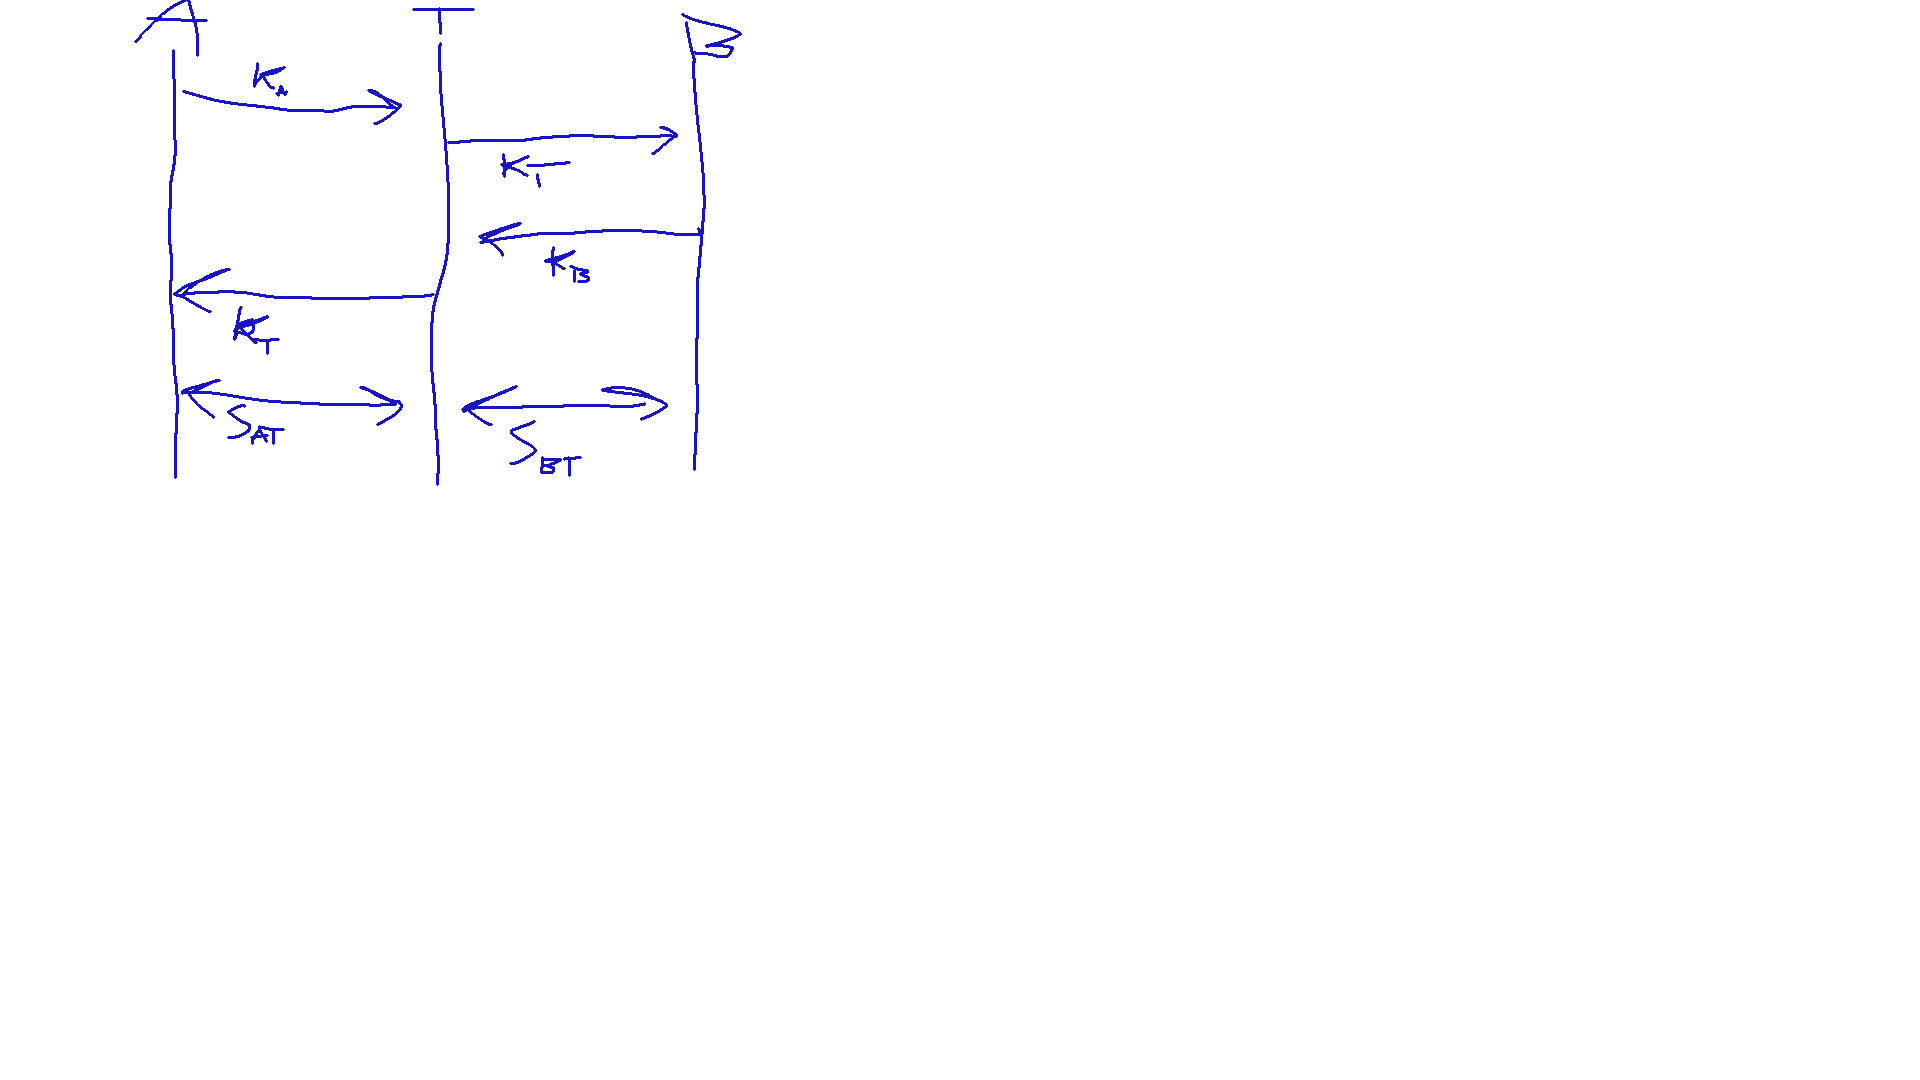
\includegraphics{coms486/hw2/Untitled.png}
    \end{question}

    \begin{question}
        \begin{enumerate}
            \item Bob request connection with Alice
            \item Alice response with her certificate
            \item Bob verifies certificate with SA
            \item Bob sends his certificate to Alice
            \item Alice verifies certificate with SA
            \item Alice randomly generates a AES key encrypts it with Bobs public key and sends it to Bob
            \item Bob decrypts AES key from Alice
            \item Alice uses AES key to encrypt sections of the file and send them to Bob
            \item Bob uses AES to decrypt file sections an save them
            \item Alice hashes whole file, encrypts the hash with her private key
            \item Alice then creates a message with that signed hash and the name of the hash function she used 
            \item Alice sends message encrypted with AES key
            \item Bob hashes file with function set by alice and compares it to value gotten from decrypting alices hash
            \item if values don't match then consider F to be tampered with and start over.
        \end{enumerate}
    \end{question}

\end{document}
